\documentclass[10pt,a4paper]{report}
\usepackage[utf8]{inputenc}
\usepackage[english]{babel}
\usepackage[T1]{fontenc}
\usepackage{amsmath}
\usepackage{amsfonts}
\usepackage{graphicx}
\usepackage{lmodern}
\usepackage{amssymb}
\usepackage{verbatim}
\usepackage{float}
\usepackage{minitoc}
\usepackage{amsthm}
\usepackage{hyperref}
\title{\LARGE{Forensics Cyber Security} \\ \vspace{0.5cm} \normalsize{Summary}}
\date{}

\begin{document}
\maketitle
\tableofcontents

\chapter{Investigation Process}
\begin{figure}[H]
\centering
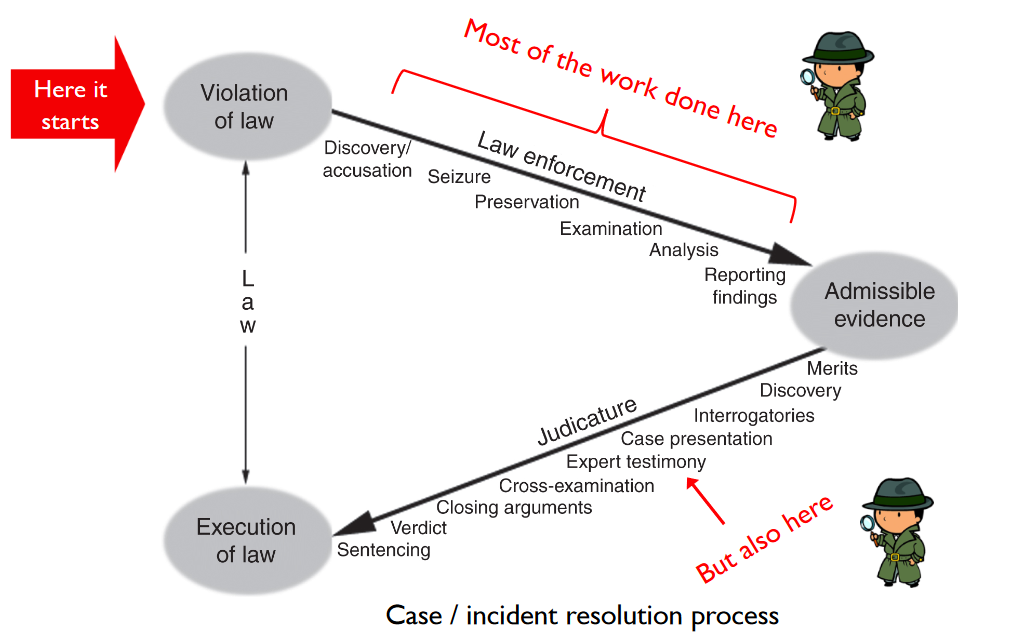
\includegraphics[scale=0.5]{1.png}
\end{figure}
\section{Investigation Models}
An investigation model is a predefined pattern of activities when performing an investigation to generate admissible evidence. The four main guidelines for admissibility of digital evidence is that it must be relevant, authentic, credible and collected legally.
\subsection{Kruse and Heiser (2001)}
Is the \textit{de facto} model used today
\begin{figure}[H]
\centering
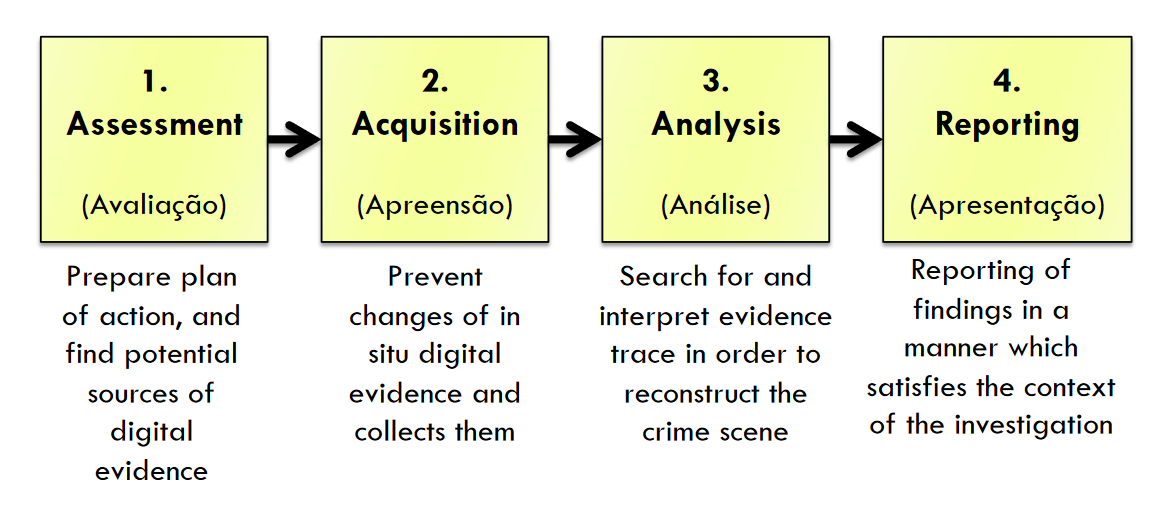
\includegraphics[scale=0.4]{2.png}
\end{figure}
\subsubsection{Assessment}
This step consists of defining the scope and likely venue of the examination, the stakeholders, the likely sources of evidence, the forensic tools, personnel and legal documentation required.\\
\\
The authorization level is set by the investigation type:
\begin{itemize}
\item Internal investigations are sponsored by an organization
\item Civil investigations require the involvement of courts
\item Criminal investigations involve the courts
\end{itemize}
For internal investigations, a signed letter of agreement outlining the scope of the investigation along with contractual details is needed. For civil and criminal investigations, a court order is needed prior to starting.
\subsubsection{Acquisition}
This step consists of acquiring and preventing changes to possible evidence. Some highlights include:
\begin{itemize}
\item Maintaining a chain of custody
\item Generating integrity checks
\end{itemize}
\subsubsection{Analysis}
In this step, the artifacts obtained in the last step are analysed in order to extract all material evidence. It is common practice to reconstruct events (temporal, relational and functional).
\subsubsection{Reporting}
The final step consists of generating the work product of the analysis, documentation. The 5 levels of documentation are:
\begin{itemize}
\item General case documentation
\item Procedural documentation
\item Process documentation
\item Case timeline
\item Evidence chain of custody
\end{itemize}
\subsection{The Scientific Method}
In practice, digital investigators need to complement investigative models with a methodology that guides them in the right direction, allows them to maintain the flexibilidy to handle diverse situations and preserves the rigors of forensic science.
\begin{itemize}
\item Observation
\item Hypothesis
\item Testing
\item Conclusion
\end{itemize}
\section{Acquiring Evidence}
When acquiring digital evidence, the main concern is to preserve it in a way that it maintains an accurate representation of the original data and that it is as complete as possible.\\
\\
The general procedure when finding storage devices it to collect them or, if they can't be taken, perfrom data extraction on the spot. When extracting data, one must be careful as to not perform any writes, usually by using a software or hardware write blocker.\\
\\
Sometimes it will not be possible to obtain an exact physical copy, bit by bit, of the entire source device, due to accessibility, space or time constraints. In this case, one can try to perform a logical acquisition of files (selecting and copying only relevant files) or volumes ( copying the contents of an encrypted volume that is being used, unencrypted, on a powered computer)
\begin{figure}[H]
\centering
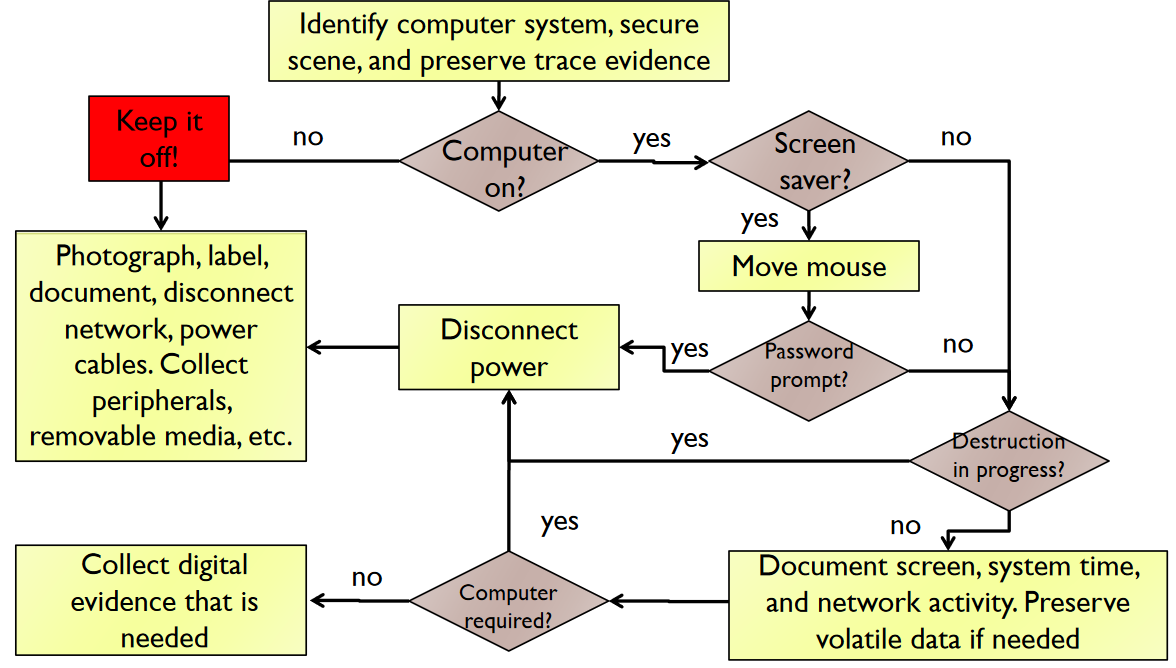
\includegraphics[scale=0.4]{3.png}
\end{figure}
\subsubsection{Mobile Devices}
Mobile devices are unique since persistent memory can't be removed and requires the original OS to be read. In this case, one should bring the device, along with power and data cables.\\
\\
If the device is powered on, it should be isolated as soon as possible, by activating airplane mode, removing sim cards or placing it inside a Faraday bag.
\section{Analysing Data}
\subsection{Data Encoding}
ASCII is the common code text representation, however, there are some ASCII extensions made to support more characters, such as UTF-8, UTF-16 or UTF-32.\\
\\
Sometimes it may also be necessary to encode binary objects into text. Base64 is a popular encoding scheme.
\subsubsection{Decoding Unknown Files}
File types have defined magic numbers, constant numerical or text value used to identify a file format or protocol. In cases where the file is corrupted certain bytes may have to be altered in order to repair it.

\chapter{Recovering Hidden Artifacts}
\section{Steganography}
Steganography is the art and science of communicating in a way that hides the existence of a message. Digital steganography works by encoding secret bits in files, such as photos or audio files, with secret data.
\subsection{Least Significant Bit}
Using this method, only the LSB of a pixel is used to encode information. More bits can be used in order to hide more information, but using too many can visually corrupt the image. Encoding on a single higher bit can be used to create a watermark.\\
\\
When using LSB, one can use consecutive pixels or take advantage of a (fixed or random) interval.
\subsection{Steganalysis}
Steganalysis is the art and science of detecting hidden data. It's methods rely on the inspection of file properties or contents and the detection of signature patters. Some approaches consist of:
\begin{itemize}
\item Visual attacks
\begin{figure}[H]
\centering
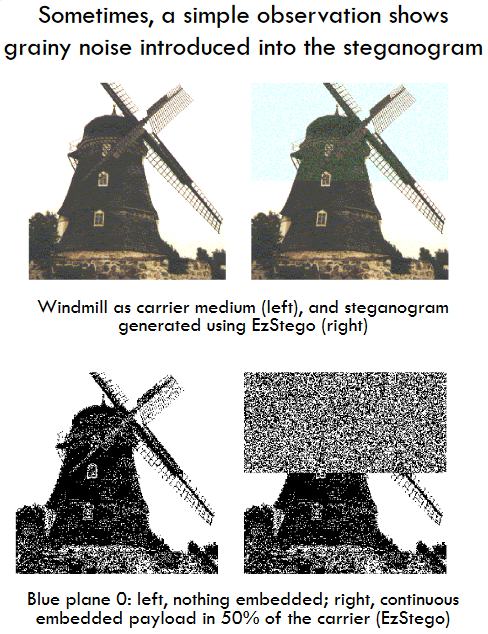
\includegraphics[scale=0.4]{4.png}
\end{figure}
\item Statistical attacks
\begin{figure}[H]
\centering
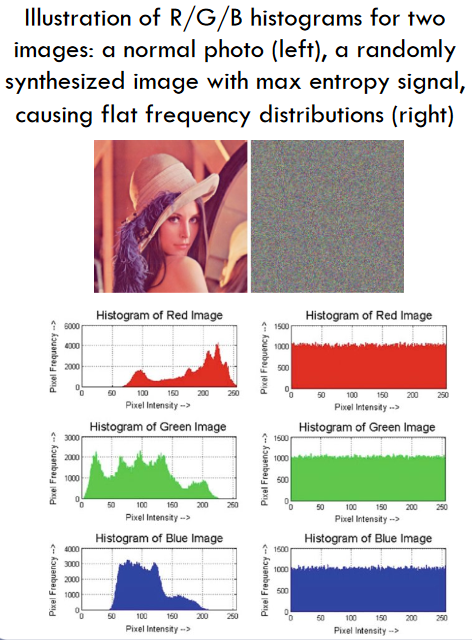
\includegraphics[scale=0.4]{5.png}
\end{figure}
\item Machine Learning
\end{itemize}
\section{Watermarking}
Watermarking is about establishing identity/ownership of digital content to prevent unauthorized use.
\subsection{LSB Embedding}
Watermarks can be applied using LSB, as mentioned before, or a higher bit in order to make it visible.
\begin{figure}[H]
\centering
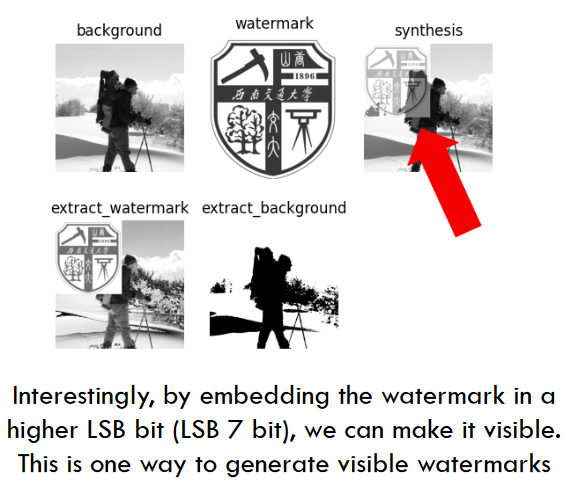
\includegraphics[scale=0.5]{6.png}
\end{figure}
\subsection{Common Investigation}
Watermarks are frequently used in proprietary content that should not be altered. If such a file is tampered with, even if the changes are not directly visible, they will likely reflect on the hidden watermark.
\begin{figure}[H]
\centering
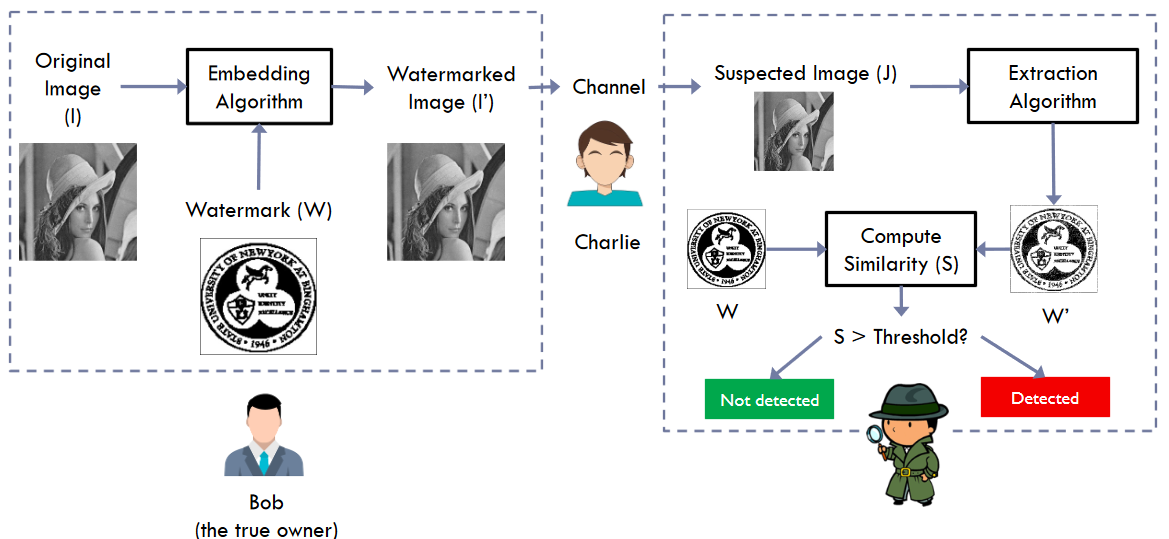
\includegraphics[scale=0.4]{7.png}
\end{figure}
\subsection{Steganography vs. Watermarking}
\begin{figure}[H]
\centering
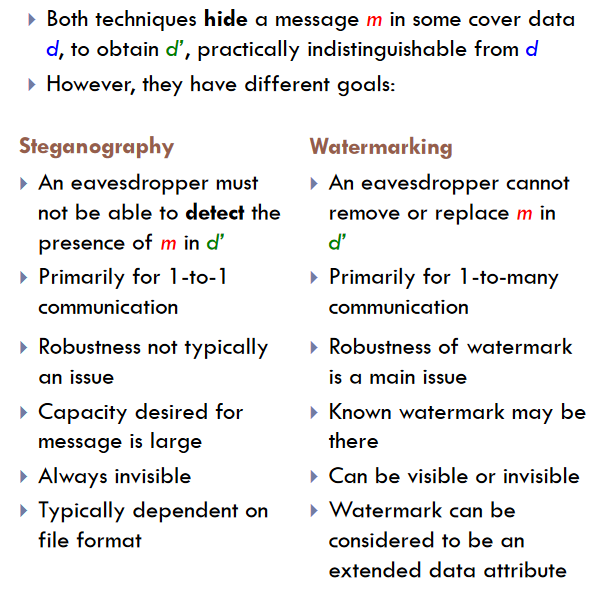
\includegraphics[scale=0.5]{8.png}
\end{figure}
\section{Memory Analysis}
Physical memory dumps may be analysed in order to recover relevant data.
\subsection{Memory Acquisition}
There are several software and hardware memory acquisition techniques. The two main factors can be used to help make a decision are:
\begin{itemize}
\item Atomicity: how close to the present memory state can the forensic memory snapshot be retrieved
\item Availability: whether the tools necessary to perform memory acquisition are available or not
\end{itemize}
Some software-based approaches include crash dumps, the hibernation fole, operating system injection and virtual machine imaging. As for hardware-based approaches, there are harware cards that can obtain forensic image of a computer’s RAM and special buses that can read volatile memory. It is also important to note the difference between warm and cold boots, since RAM retains memory during reboots as long as power is provided:
\begin{itemize}
\item Warm boots refer to reboot methods in which power is never removed from the memory module (e.g., press reset button)
\item Cold boot refers to reboot methods in which power is removed from the memory module (e.g., pull the plug and reboot)
\end{itemize}
\subsection{Virtual Addresses}
Virtual addresses may be converted into physical addresses, like the following example:
\begin{figure}[H]
\centering
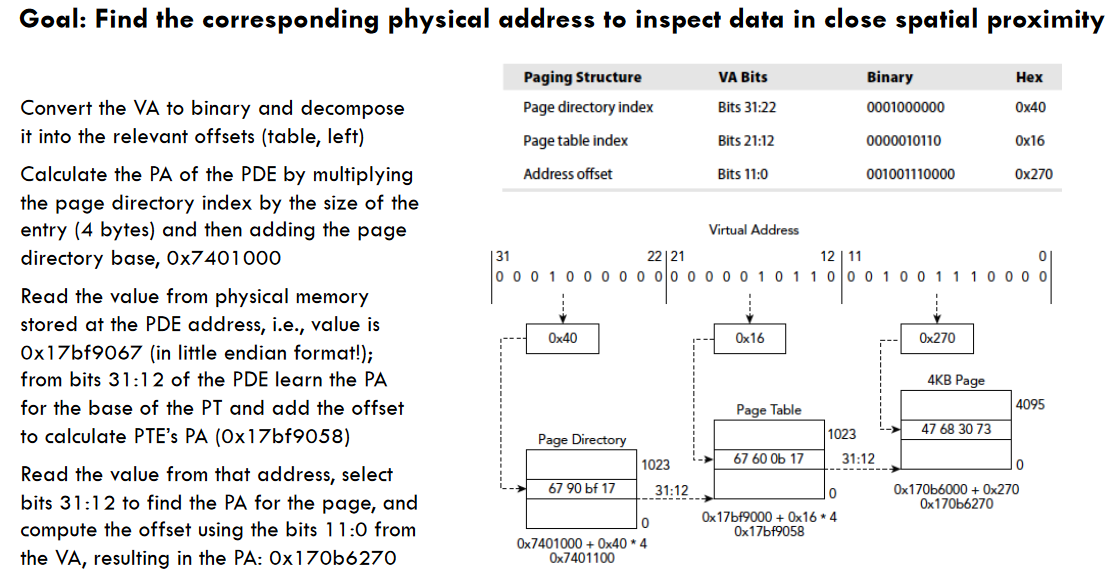
\includegraphics[scale=0.5]{9.png}
\end{figure}
\subsection{Forensic Interpretation of Memory Dumps}
Once a memory dump has been performed, it is necessary to interpret the data structures in the raw memory sample. Some methods used include:
\begin{itemize}
\item Tree/list traversal: find index into lists/trees of interest and follow them through pointer dereferencing to reconstruct the full data structure
\item Fingerprint/pattern search: search for relevant patterns in memory
\end{itemize}
\subsection{Identifying Malicious Processes and Network connexions}
Upon capturing a RAM dump, it is possible to list all the active processes and network connextions, making it possible to indentify and extract malicious code.
\section{Storage And Volume Analysis}
A volume is a collection of addressable sectors that an OS or application can use for data storage. A partition is a fraction of consecutive sectors in a volume. By definition, a partition is also a volume.\\
\\
\subsection{Layout}
To identify the volume layout, the partition tables must be analyzed, however if the partition system becomes corrupt or erased, automated tools may not work.
\subsubsection{Consistency}
It's necessary to check  each partition relative to the other partitions.
\begin{figure}[H]
\centering
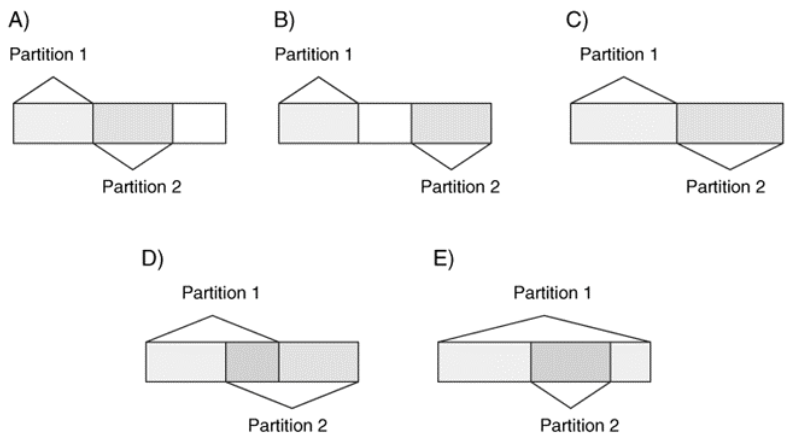
\includegraphics[scale=0.5]{10.png}
\end{figure}
\subsection{HDD And SSD}
There are some considerations of note when working with different drive types.
HDDs can have passwords, be self-encrypting or self-wiping. It is possible to hide data in the Host Protected Area (HPA), added in ATA-4 spec. There are also two types of formatting for these drives:
\begin{itemize}
\item Low-level formatting: Physically defines tracks and sectors on disk and erases data
\item High-level formatting: Performed when initializing a file system on a partition, does not destroy data, only FS metadata
\end{itemize}
SSDs are not as well understood ad HDDs, the physical location of data is hard to predict, deleted data is hard to recover and it is difficult to read data off chips directly.
\subsection{Evidence From File Systems}
Each partition of a disk can have its own file system. In many Linux distributions, ExtX is the default file system. In ExtX:
\begin{itemize}
\item File contents are stored inside blocks
\item The blocks allocated to a file are kept by a record called inode
\item Directory entries associate the file name with the file’s inode
\end{itemize}
\begin{figure}[H]
\centering
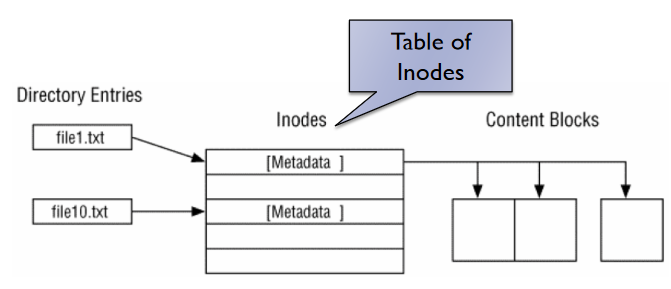
\includegraphics[scale=0.5]{11.png}
\end{figure}
Each inode is the root of an unbalanced tree of blocks that belong to a given file. To keep track of inode and block allocation bitmaps (bit arrays) are used. The inode bitmap tells which inodes are allocated to files and the block bitmap tells which data blockas are allocated to files.
\begin{figure}[H]
\centering
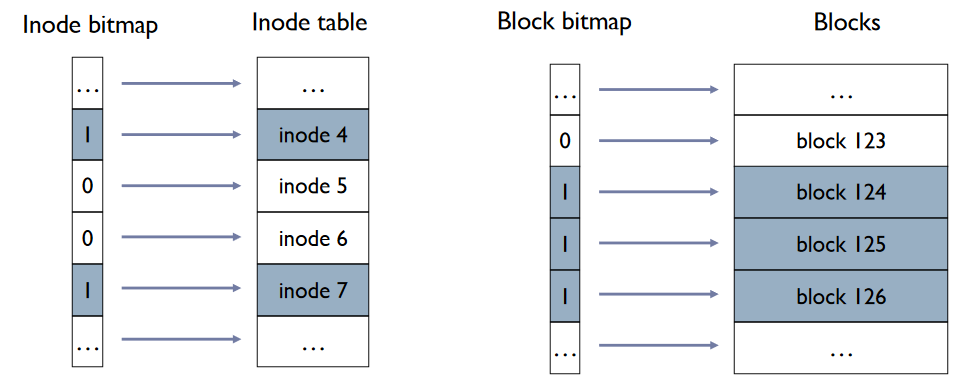
\includegraphics[scale=0.4]{30.png}
\end{figure}
In order to create a new file it's necessary to allocate a new inode, the required blocks and an entry in the directory, as well as update data blocks, inode, and directory entry. When deleting a file, the inode and block bitmaps are updated and the directory entry unallocated, most contents of inode, data blocks, and directory entry remain intact. Deleting a file involves updating the record length of previous file entry in the directory.\\
\\
In Ext3, the recent history of updates to the system is mantained in a journal. Journals are implemented as a circular buffer and are append-only. If the computer crashes while journaling, the file system may enter an inconsistent state.\\
\\
The ExtX file system is organized as sequence of logical blocks in disk (block size is defined upon disk formatting). Blocks are grouped into larger units called block groups and all block groups have equal length possibly except the last one. The first data block aka boot block is not used by the FS, it has a fixed 1024 byte length and may contain bootstrap code.
\begin{figure}[H]
\centering
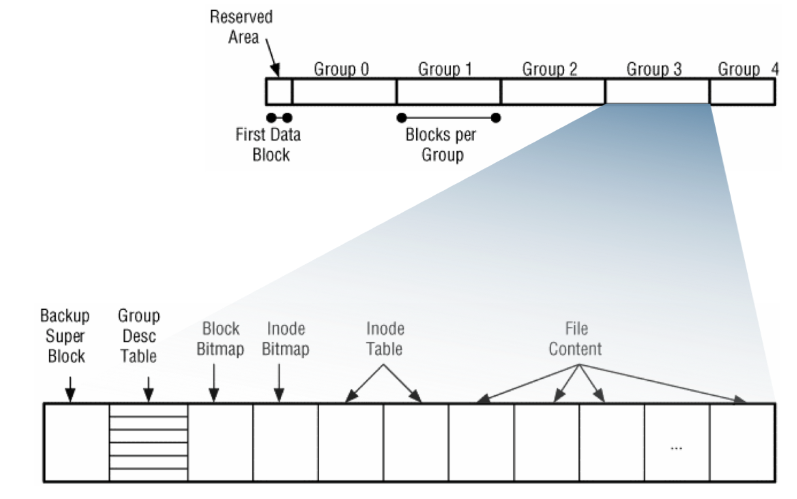
\includegraphics[scale=0.5]{31.png}
\end{figure}
Data evidence categories of the ExtX file system family:
\begin{figure}[H]
\centering
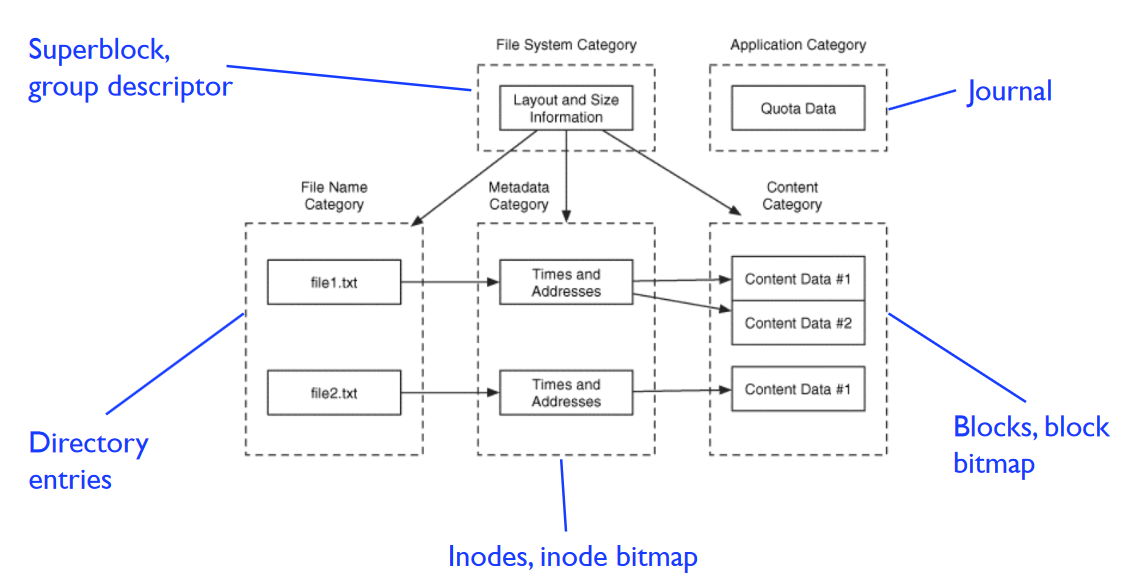
\includegraphics[scale=0.4]{12.png}
\end{figure}
\subsubsection{File System Analysis Techniques}
In the content category:
\begin{itemize}
\item Data unit viewing
\item Logical file system-level searching
\item Unallocated data unit searching
\item Consistency analysis
\item Data carving
\item Anti-forensic techniques (e.g., data wiping)
\end{itemize}
In the metadata category:
\begin{itemize}
\item Metadata lookup
\item Logical file viewing
\item Logical file searching
\item Unallocated metadata analysis
\item Metadata attribute searching and sorting
\item Consistency checking
\end{itemize}
In the file name category:
\begin{itemize}
\item File name listing
\item File name searching
\item Consistensy checking
\end{itemize}
\subsubsection{NTFS}
In NTFS, files are chunked into clusters (akin to ExtX's blocks), with the central paradigm that everything is a file.
\begin{figure}[H]
\centering
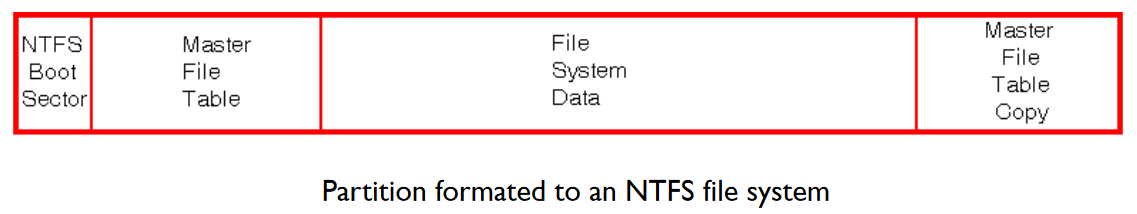
\includegraphics[scale=0.5]{34.png}
\end{figure}
In NTFS, information about all files and directories is contained in the Master File Table (MFT). Every file and directory has at least one entry in MFT (1kb size).
\begin{figure}[H]
\centering
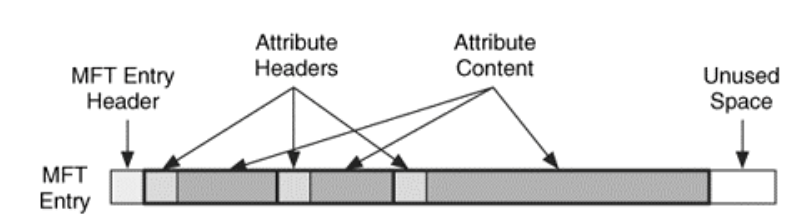
\includegraphics[scale=0.5]{35.png}
\end{figure}
MFT entries are a precious source of forensic data and some small files can fit entirely within the MFT entry, bigger files require allocation of extents. NTFS stores metadata across several metadata files. Steps for file creation:
\begin{itemize}
\item Find an unallocated MTF entry for the new file (304)
\item Initialize the MFT entry 304 with basic attributes
\item Allocate two clusters in the \$BITMAP file (692, 693)
\item To add a file name, first look up the root directory
\item Then, locate the dir1 index in the directory’s B-tree
\item Follow the entry address 200, and add index entry for file1.txt
\item In previous steps, add entries to journal
\end{itemize}
And to delete a file:
\begin{itemize}
\item Find the dir1 directory by processing the MFT entry 5, the root directory
\item Search for the file1.dat entry, whose address is 304
\item Remove the entry from the index of dir1
\item Unallocate MFT entry 304 by cleaning the in-use flag
\item Clusters of entry 304 unallocated in the \$Bitmap file
\item In previous steps, add entries to journal
\end{itemize}
In NTFS, every file has a \$DATA attribute, which contains the file content. However, a file can have more than one \$DATA attribute, named Alternate Data Stream (ADS). ADSs are great for hiding files inside files, without creating a new MFT entry.
\subsection{File Carving}
File carving is a powerful technique because it can identify and recover files of interest from raw, deleted or damaged file systems, memory, or swap space data. There are different techniques, such as:
\begin{itemize}
\item Structure-based carving (e.g. magic numbers)
\item Content-based carving
\end{itemize}
\subsubsection{Parallel Unique Path (PUP)}
The key insight behind the PUP algorithm is to grow all files simultaneously and append best match at each step.
\begin{itemize}
\item Initially, assume that all file clusters are randomized and identifies headers using keywords/signatures
\item For each header, find best match (using matching metric)
\item Find best match for recently added node
\item Repeat until all files are built or no more nodes can be chosen
\end{itemize}
\subsubsection{Bifragment Gap Carving (BGC)}
BGC leverages an observation that bifragmentation (two fragments only) is the most common fragmentation type. Its goal is to match both fragments of each file.\\
\\
It uses magic number to locate the header and footer and, to verify if they are properly sequenced, checks if the file obeys the structured rules of its file type.
\section{Evidence In Operating Systems}
OS artifacts are evidentiary data pertaining to data/code maintained/executed by the OS. Such artifacts can help track past/live user activity
\begin{figure}[H]
\centering
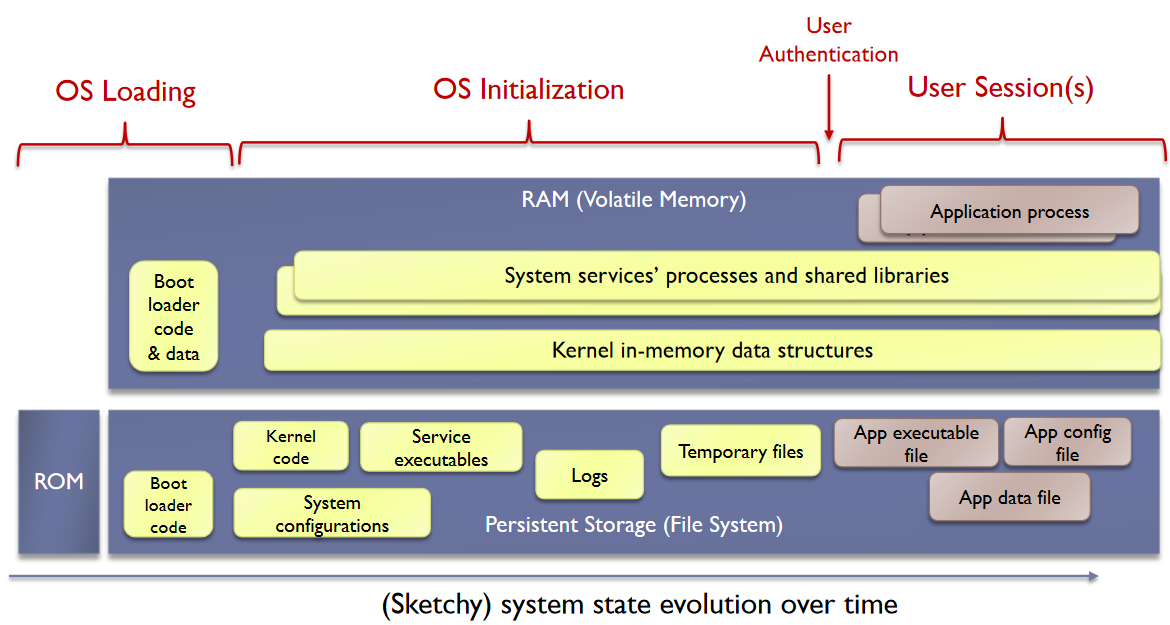
\includegraphics[scale=0.4]{13.png}
\end{figure}
Some typical user activities to investigate include:
\begin{itemize}
\item File download
\item Program execution
\item File opening/creation
\item Deleted file or file knowledge
\item Physical device location
\item USB or drive usage
\item Account usage
\item Network usage
\end{itemize}
\subsection{Location of Artifacts}
The location of artifacts is OS-dependent.
\begin{figure}[H]
\centering
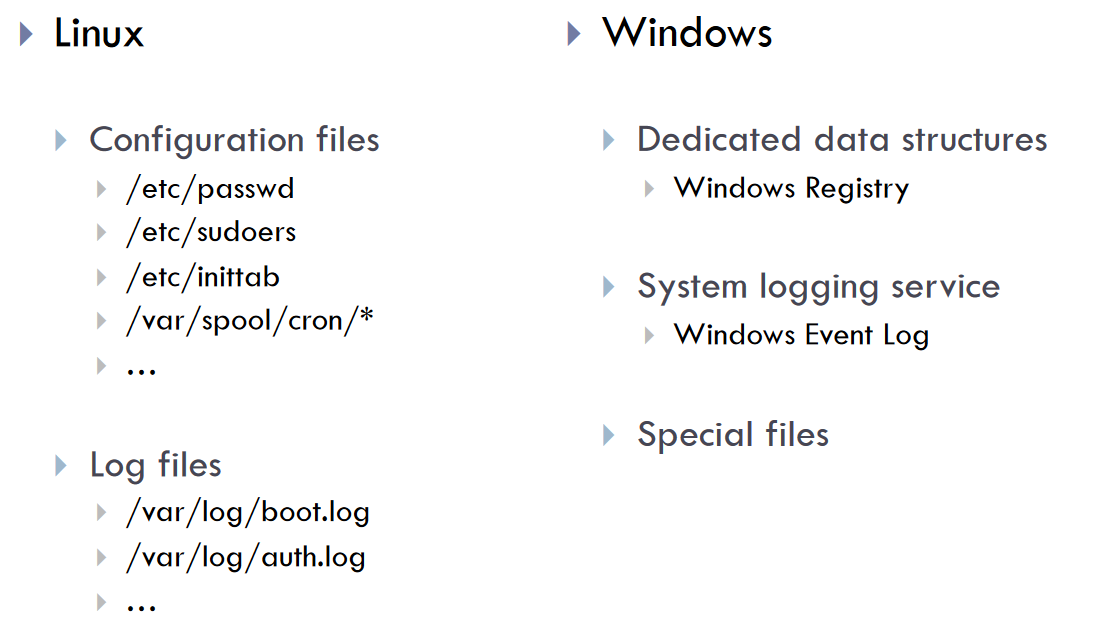
\includegraphics[scale=0.4]{14.png}
\end{figure}
\subsubsection{Windows Registry}
Virtually everything done in Windows refers to or is recorded into the registry. The Registry can be seen as a unified file system, its specific structure is divided into keys and values. Main root keys (named hives) represent the root directory, sub-keys represent the sub folders, and values represent the files.
\begin{figure}[H]
\centering
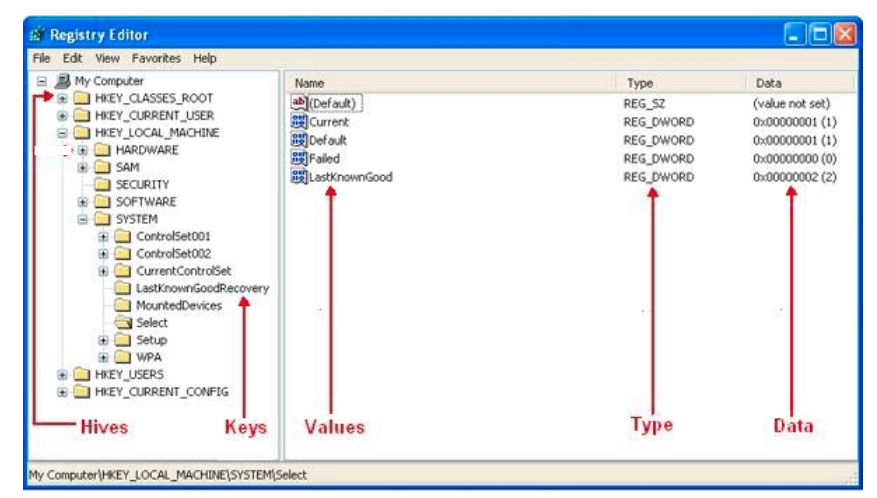
\includegraphics[scale=0.4]{15.png}
\end{figure}
The registry is commonly described as a hierarchical database, however, its database is only ever complete when loaded into your computer's memory, and it is the sum  of two parts, the data and the processes that create it and provide access to it.
\begin{figure}[H]
\centering
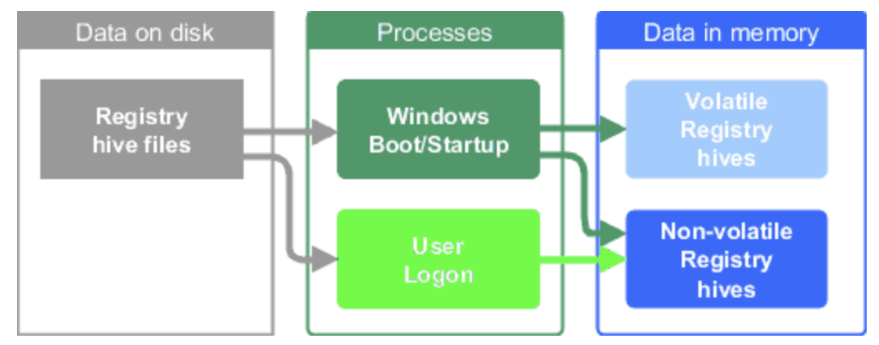
\includegraphics[scale=0.3]{16.png}
\end{figure}
Each root key shown in the registry editor is actually a file in the filesystem called registry hive. A hive contains a logical group of keys, subkeys, and values in the registry that has a set of supporting files containing backups of its data.
\begin{figure}[H]
\centering
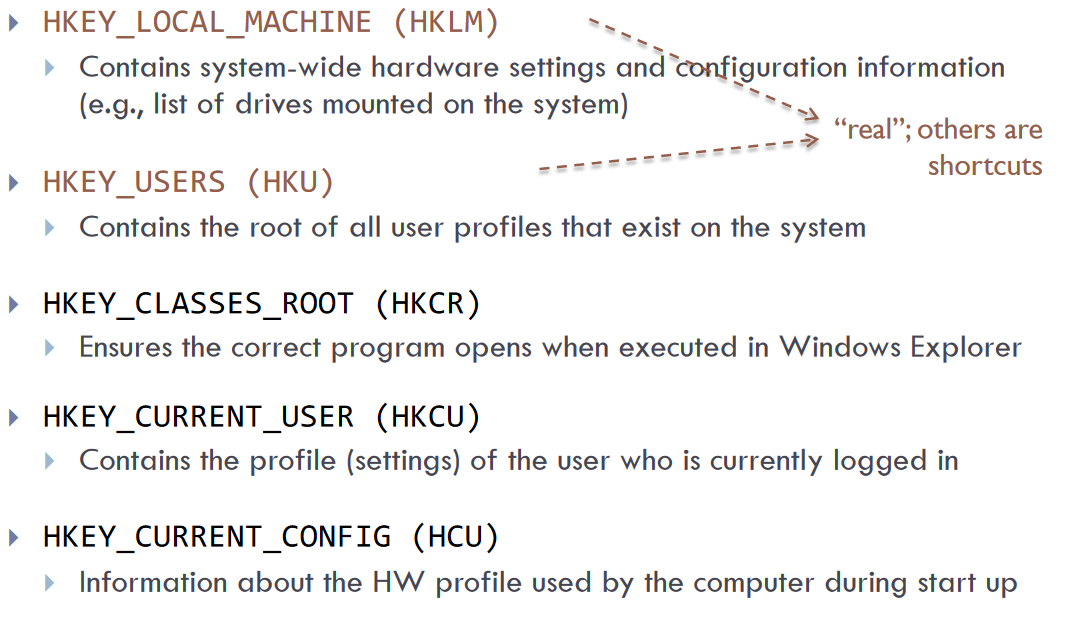
\includegraphics[scale=0.4]{36.png}
\end{figure}
Some registry hives are stored on disk even
when Windows is not running. All the registry hive structures only exist in memory. This includes a set of volatile hives that only exist when Windows is running. Access is done through the Registry
Configuration Manager.
\subsubsection{Windows Event Log}
Whenever an event, such as a user logging on or off, occurs, the operating system logs the event. Windows has a centralized log service to allow apps and OS to report events that have taken place.
\begin{figure}[H]
\centering
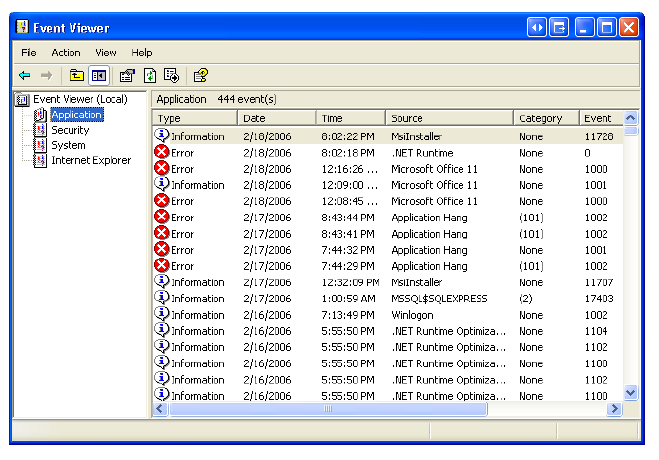
\includegraphics[scale=0.4]{17.png}
\end{figure}
Some other interesting artifacts include:
\begin{itemize}
\item MRU lists: MRU ('most recently used') lists contain entries about specific actions done by the user
\item OpenSave MRU:  tracks files that were opened / saved within a Windows shell dialog box
\item Last Visited MRU: Tracks the specific executable used by an application to open the files documented in the OpenSaveMRU key
\item UserAssist: contains information about the exe files and links that you open frequently
\item Shell Bags: track user window viewing preferences to Windows Explorer
\item Prefetch files: a prefetch file is created when an application is run from a particular location for the very first time; used to speed up the loading of applications
\item Thumbnails: (on Win XP) hidden file thumbs.db in directory where pictures exist; stores thumbnail even if pictures deleted
\item Autorun locations: registry keys that launch programs or apps during boot
\end{itemize}
\section{Time Tracking}
Computers have several different methods of timekeeping:
\begin{itemize}
\item Real Time Clock (RTC)
\item System clock
\item Network Time Protocol (NTP)
\item Network Identity and Time Zone (NITZ)
\item Global Positioning System (GPS)
\end{itemize}
Timestamps may not always be reliable, due to bugs, synchronization issues, bad configurations or interpretation, etc.
\subsection{Time Tracking In File Systems}
MACtimes are three time attributes attached to any file or directory in UNIX, Windows, and other systems:
\begin{itemize}
\item atime: last time the file or directory was accessed
\item mtime: changes when a file’s contents are modified
\item ctime: keeps track of when the contents or meta-data about the
file has changed: owner, group, file permissions, etc.
\end{itemize}
Sometimes this information is enriched with creation time.
\subsection{Timestomping}
Timestamps are not meant to be manipulated by the end user, however, a resourceful user (and often, malware) can modify these timestamps using various methods: this is called timestomping. Some strategies for timestomping detection include:
\begin{itemize}
\item Anomalies in timestamp format
\item Inconsistencies between MFT attributes
\item Inconsistencies with other timing sources
\end{itemize}
\subsection{Digital Stratigraphy}
Digital stratigraphy is a new sub-field emerging in digital forensics that studies file system traces and writing patterns to infer time-related facts. This is usually:
\begin{itemize}
\item Based on how data was overwritten:
\begin{figure}[H]
\centering
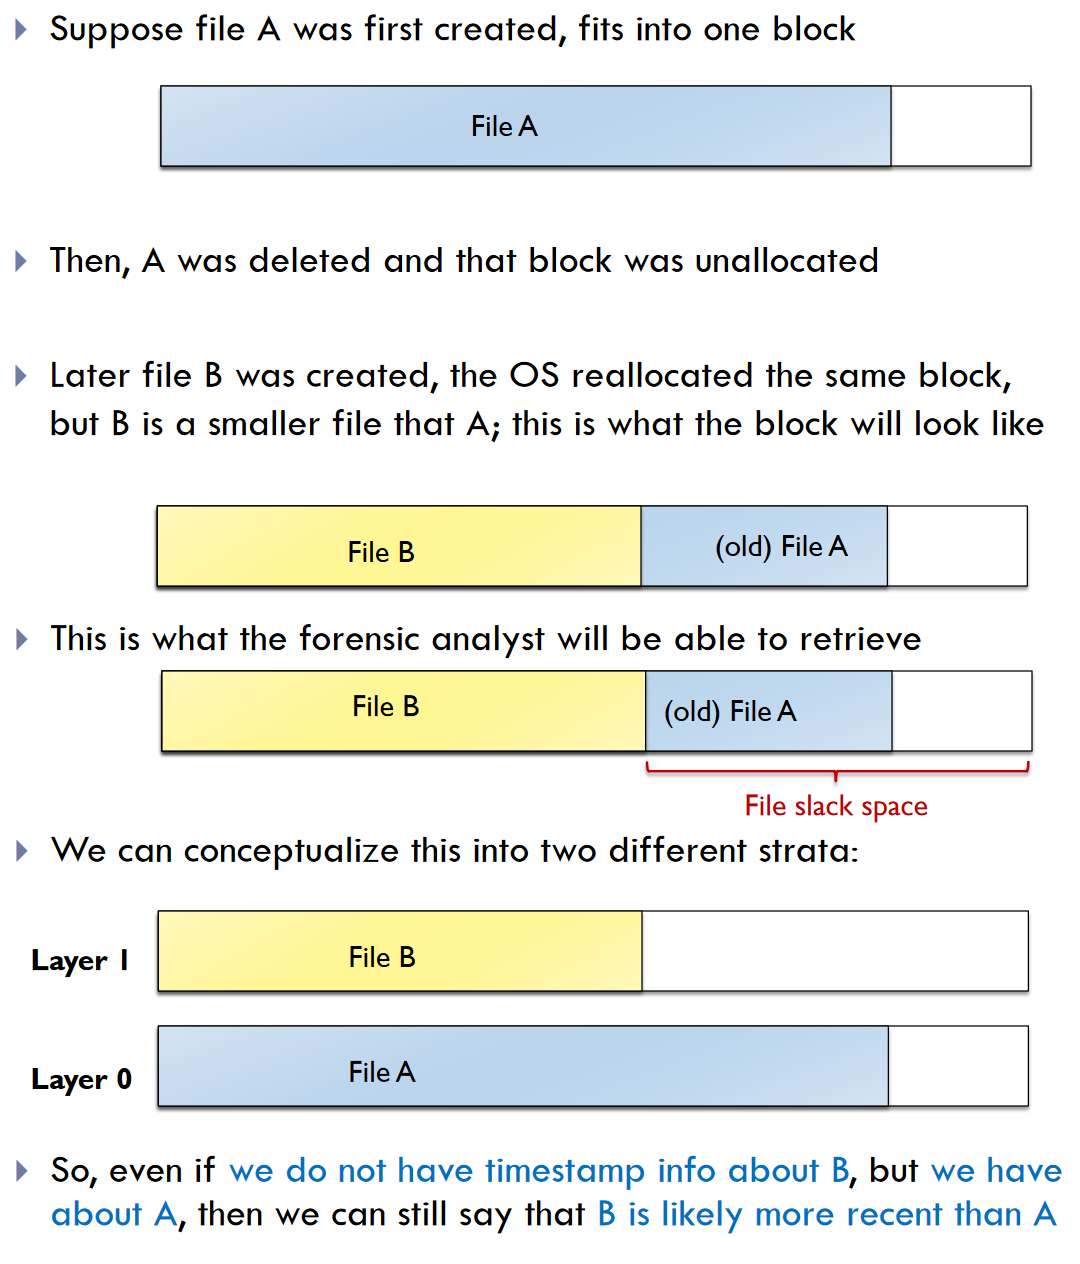
\includegraphics[scale=0.3]{18.png}
\end{figure}
\item Based on data positioning:
\begin{figure}[H]
\centering
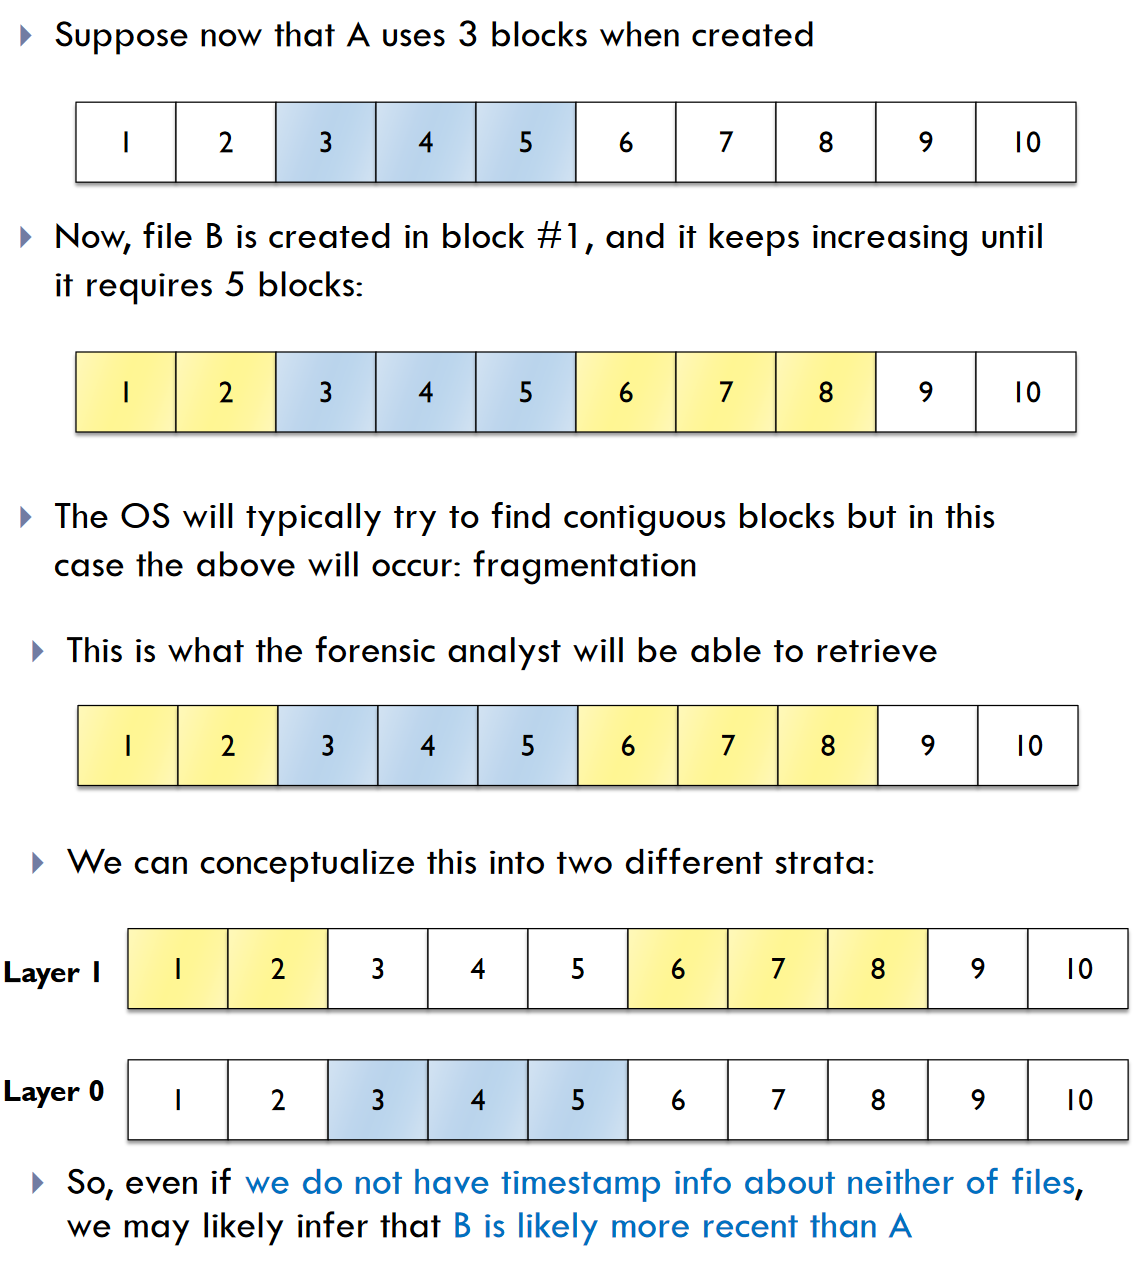
\includegraphics[scale=0.3]{19.png}
\end{figure}
\end{itemize}
\section{Network Traffic Analysis}
The analysis of network traffic allows us to collect information from network traces and detect potential attacks and inspect the contents of communications.
\subsection{Packet Analysis Techniques}
Packet traces are usually collected through packet sniffers. Some of the main packet analysis techniques include:
\begin{itemize}
\item Parsing protocol fields
\item Packet filtering
\item Pattern matching
\end{itemize}
\subsection{Flow Analysis Techniques}
A flow is a sequence of packets sent from a particular source to a particular unicast, anycast, or multicast destination that the source desires to label as a flow. Flow analysis consists in examination of sequences of related packets. The usual techniques include:
\begin{itemize}
\item List flows
\item Export a flow
\item File and data carving
\end{itemize}
\subsubsection{NetFlow}
NetFlow is a technology built into supported devices that collects and categorizes IP traffic, but does not collect the entire payload of the packets. It logs flows, not TCP connections, and for each TCP connection two flows are recorded (since flows are uni-directional).
\subsection{Protocol Analysis Techniques}
Protocol analysis aims to understand how a particular communications protocol works, what it’s used for, how to identify it, how to dissect it. Many protocols are standardized, but many others are deliberately kept secret. Some techniques include:
\begin{itemize}
\item Search for common binary/hexadecimal/ASCII values that are typically associated with a specific protocol
\item Leverage information in the encapsulating protocol
\item Leverage the TCP/UDP port number, many of which are associated with standard default services
\item Analyze the function of the source or destination server (specified by IP address or hostname)
\item Test for the presence of recognizable protocol structures
\end{itemize}
\section{Pitfalls in Network Addressing}
Network addressing includes MAC and IP addresses, as well as port numbers, which may not always be reliable.
\subsection{MAC addresses}
A MAC address is a unique identifier assigned to network interfaces for communications at the
data link layer of a network segment. It can be used to track traffic sources within a network, but  it can be modified, so one must be careful about using it as a unique identifier.
\subsection{IP addresses}
IP addresses are scope-defined, and thus, private IP addresses can't be routed through the internet, and are only meaningful on its private network.\\
\\
One of the main sources of unreliability of IP addresses is the risk of spoofing of the source IP, which might be unreliable in unidirectional communication.\\
\\
IP addresses may also be masked by middleboxes, such as proxies, VPN servers, NAT, load balancers or firewalls. Some protocols, such as IPsec, also implement tunneling to mask the IP until reaching its final destination.
\subsection{Ports}
Certain protocols have defined ports for communication. Internet Assigned Numbers Authority (IANA) is responsible for IP addresses and port number assignments for well-known ports.\\
\\
A technique called port knocking aims at hiding ports from view. To gain access to the service you want, you need to go through what amounts to a network authentication. A method of externally opening ports on a firewall is by generating a connection attempt on a set of prespecified closed ports
\section{Network Scanning}
Network scanning is concerned with determining the topology of a given network.
\subsection{Traceroute}
Traceroute is a very useful tool for network scanning. It works by making use of the time to live (TTL) IP header field. It works by:
\begin{itemize}
\item Sending a message out to a destination with increasing TTL values
\item The first packet being sent has a TTL of 1
\item When the very first router (the default gateway) receives the message, it decrements the TTL to 0 and responds with the ICMP error message
\item Once the sending system receives the message, it has the IP of the first router
\end{itemize}
\subsection{Nmap}
Nmap is useful in order to get open TCP ports. It works by performing a SYN scan. A system that has an open port will respond with the SYN/ACK or with a RST message. Nmap responds with a RST after the SYN/ACK.\\
\\
Nmap can also perform other scan types, such as connect, FIN and UDP scans.
\subsection{Other Techniques}
\subsubsection{Banner Grabbing}
It’s the process of connecting to a service and probing it to get the service banner. Different protocols support different ways of conveying information about themselves. One can use the netcat (nc) tool for banner grabbing.
\subsubsection{Ping Sweeps}
A ping sweep is a way of identifying all of the hosts that are discoverable on a network. We can use what nmap calls host discovery.
\subsubsection{Vulnerability Scanners}
A vulnerability scanner works with a database of signatures, and this database needs to be updated regularly.
\subsubsection{Network Intrusion Detection Systems}
Such systems may provide alerts or logs that include details regarding illicit connextions, and can be configured to begin detecting events it wasn’t previously recording.
\subsection{Correlating Events Across the Network}
Individual pieces of digital data might not be useful on their own, but patterns may emerge when combined. To develop a clearer picture of the crime, three forms of reconstruction should be performed when analyzing evidence:
\begin{itemize}
\item Relational (who, what, where)
\item Temporal (when)
\item Functional (how)
\end{itemize}

\chapter{Specialized Techniques and Tools}
\section{Wireless Network Forensics}
Wireless networks are important in forensic analysis since, through them, it's possible to identify and recover devices, assets or individuals.
\subsection{Man-In-The-Middle Attacks}
Free wi-fi networks are susceptible to this type of attack.\\
\\
An attacker might set up a hotspot spoofing the wi-fi network using the same SSID and password and have victims mistakenly connect to it. This is then used to listen to their traffic and possibly steal sensitive information.
\subsection{Other Typical Wi-Fi Attacks}
Some other common wi-fi attacks include:
\begin{itemize}
\item Decryption attacks: WEP is easily broken; WPA2 can be broken under week passwords
\item Wardriving: Attackers drive around a neighborhood and use a laptop with a GPS device, antenna to identify and record the location of unprotected wireless networks
\item Packet sniffing: Use packet sniffers to intercept traffic on unencrypted WiFi networks or on breakable WEP/WEP2 networks
\item Rogue access points: Unauthorized wireless APs that extend the localnetwork bypassing network-enforced security measures
\end{itemize}
\subsection{Cellular Networks and Location Tracking}
Cellular networks have the same types of forensic data as other TCP/IP networks, along with SMS and telephone calls.
\subsubsection{Identifiers}
In this type of network, two new device identifiers are present:
\begin{itemize}
\item IMEI: a unique number associated with a particular device (searchable on a database)
\item  IMSI: an identifier of a SIM card. Allows to track all activities relating to a particular subscriber.
\end{itemize}
\subsubsection{Tracking Location}
There are several positioning techniques:
\begin{itemize}
\item Proximity
\item Trilateration, Triangulation
\item Fingerprinting
\item Hybrid
\item GPS
\end{itemize}
\begin{figure}[H]
\centering
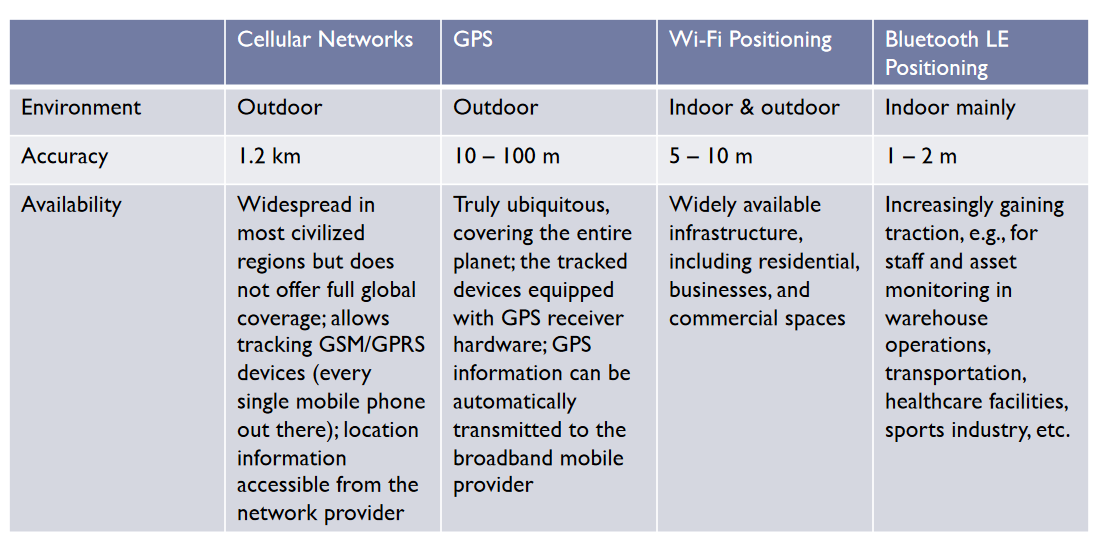
\includegraphics[scale=0.4]{20.png}
\end{figure}
\subsubsection{Attacks}
Some specific cyberattacks involving cellular networks include GPS spoofing, smishing and SIM swapping attacks.
\section{Email Forensics}
Ease, speed and relative anonymity of email makes it lucrative option for committing crimes for the criminals. Some common email attacks include:
\begin{itemize}
\item Email spamming: can be defined as sending unsolicited emails
\item Mail Bombing: the primary intention of mail bombing is to cause denial-of-service attack to the victim. It is achieved by sending huge volumes of emails to the victim's mailbox/server to crash down
\item Phishing: defined act of sending an unsolicited and illegitimate email falsely claiming to be from legitimate site/company to win the victim's trust and acquire their personal/account information
\item Email spoofing: the act of forging the email header so that the message appears to originate from source other than the actual source
\end{itemize}
\subsection{Email Investigations}
In email investigations, one looks for evidence of email abuse/incriminating content. The way such investigations are conducted is dependent on the protocols used:
\begin{figure}[H]
\centering
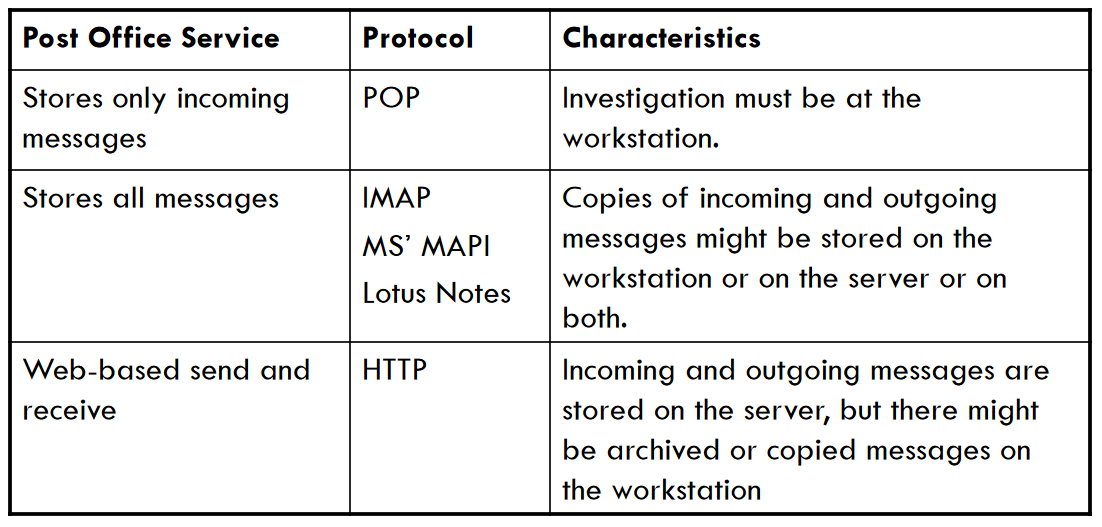
\includegraphics[scale=0.4]{21.png}
\end{figure}
Some email-related sources of evidence include the header (email itself) and the logs left behind. The header includes the sender, the network path it traversed, timestamp details, encoding information, etc.\\
\\
Some general advice is to verify IP addresses, look for breaks/discrepancies in the "Received" lines and make a timeline of events.
\subsection{Antiforensics}
\subsubsection{Open Relays}
Open relays are SMTP server configured in such a way that it allows anyone on the Internet to send e-mail through it, not just mail destined to or originating from known users.\\
\\
Spoofers use open relays to attempt to hide the person and IP of the system that sent the email. In these cases, the header and logs will contain the originating address.
\subsubsection{False Received From Header}
Such a header leads the investigator to the wrong server by adding a seemingly valid received from header. To avoid detection, the spoofer’s real address will be recorded somewhere in the Received from headers, but the investigator will not know which one.\\
\\
In these cases, email received from headers will contain the actual IP address of the originating system, you just won’t know which header is correct.
\section{Web Forensics}
An attack scenario describes the ways an attacker might exploit the vulnerabilities of a Web app. These apps are often distributed and business critical, which prove to be challenges for web investigations.
\subsection{Code Injection Attacks}
These attacks are carried out via entering malicious code into the input control of web form or address bar of web browser. Some common types are:
\begin{itemize}
\item Cross Site Scripting (XSS): XSS attacks allows an attacker to run arbitrary JavaScript in the context of a vulnerable website. The goal is to steal the client cookies or other sensitive info which can identify the client with the web site
\item SQL injection: an attacker injects malicious text string, most often a database query, into an available web form that is eventually executed by the database
\item PHP injection: allows an attacker to supply code to the server side scripting engine. This vulnerability allows an attacker to run arbitrary, system level code on the vulnerable server and retrieve any desired information contained therein.
\end{itemize}
\section{Deep Web And Anonymity}
The surface web is that portion of the World Wide Web that is readily available to the general public and searchable with standard web search engines.\\
\\
The deep web is not necessarily bad, it’s just that the content is not directly indexed. The part of the deep web where criminal activity is carried out is named the dark web.
\subsection{Google Hacking}
Google provides keywords for advanced searching, which can be used to search for file types, finding servers or even unprotected webcams.
\subsection{Anonymity}
It's hard to be anonymous on the internet:
\begin{itemize}
\item IP addresses can be linked directly to individuals
\item Browsers can be tracked
\item Activities can identify people
\item Internet access points can be wiretapped
\end{itemize}
\subsubsection{Anonynity Systems}
The aim is to conceal the identity of communicating parties. There are several types of anonymity, all with the desired properties of unlinkability and unobservability:
\begin{itemize}
\item Sender anonimity
\item Receiver anonimity
\item Sender-receiver anonimity
\end{itemize}
Anonimity can be quantified through anonimity sets, the number of suspects. The larger the set, the stronger the anonimity.
\subsection{Anonymity Networks}
The aim is to overcome limitations of public proxy servers. An anonimity network forwards traffic through a chain of network nodes: relays.
\subsubsection{Onion Routing}
Onion routing uses public-key cryptography to establish a "circuit" with pairwise symmetric keys between hops on the circuit. The sender chooses a sequence of routers and then symmetric criptography is used to move data.
\begin{figure}[H]
\centering
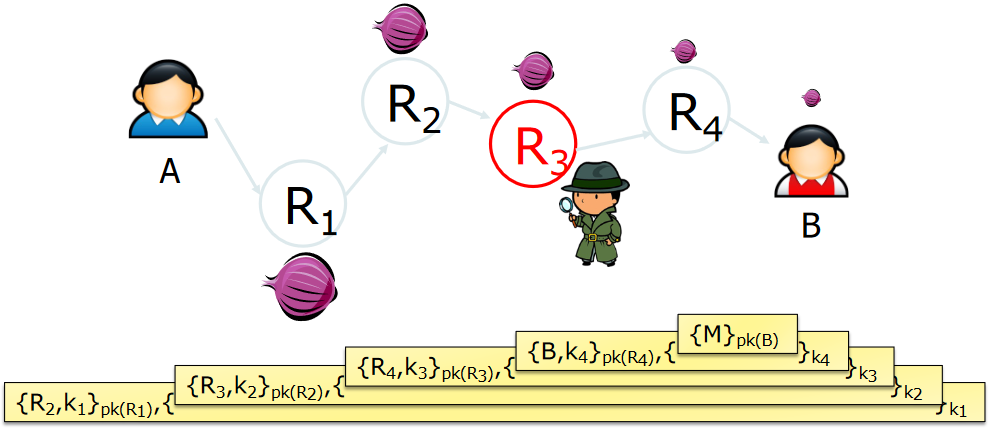
\includegraphics[scale=0.5]{28.png}
\end{figure}
Routing info for each link encrypted with router’s public key. Each router learns only the identity of the next router.
\subsubsection{Tor}
Tor is the 2nd generation onion router, a volunteer-based low-latency anonymity network. When Bob wants to connect to Alice through Tor, he downloads the Consensus (list of Tor relays) from the Tor authorities. Each Tor relay is uniquely identified by an RSA public key. Then three "random" relays are chosen, and the following circuit establishment happens:
\begin{itemize}
\item Connecting to first relay:
\begin{itemize}
\item Bob sets up a TLS connection with the Entry node
\item Negotiates a Diffie-Hellman (DH) key with first node in path
\end{itemize}
\item Connecting to second relay:
\begin{itemize}
\item Then complete a DiffieHellman key exchange handshake with the second node by using the first node as a proxy
\end{itemize}
\item Connecting to third relay:
\begin{itemize}
\item Repeat the same procedure with the third node but use the chain of entry and middle nodes as proxies
\end{itemize}
\item Data transmission:
\begin{itemize}
\item To connect to a server, the client packs the messages in fixed 512 byte cells, encrypted with the three relay keys.
\item Each relay strips off one layer of encryption, breaking the linkability between the sender and the destination
\item Normally, messages are also encrypted using end-to-end protocol
\end{itemize}
\end{itemize}
\subsection{Hidden Services And The Dark Web}
Tor supports hidden services: allows for running a server and have people connect without disclosing the IP or DNS name. This is done through a rendezvous point: a meeting place for the user and service.\\
\\
Each hidden service has introduction points (yellow), that can be found through Onion URLs, since they are hashes. Before sending an introduction message, the client selects a rendezvous point, and then informs the service:
\begin{figure}[H]
\centering
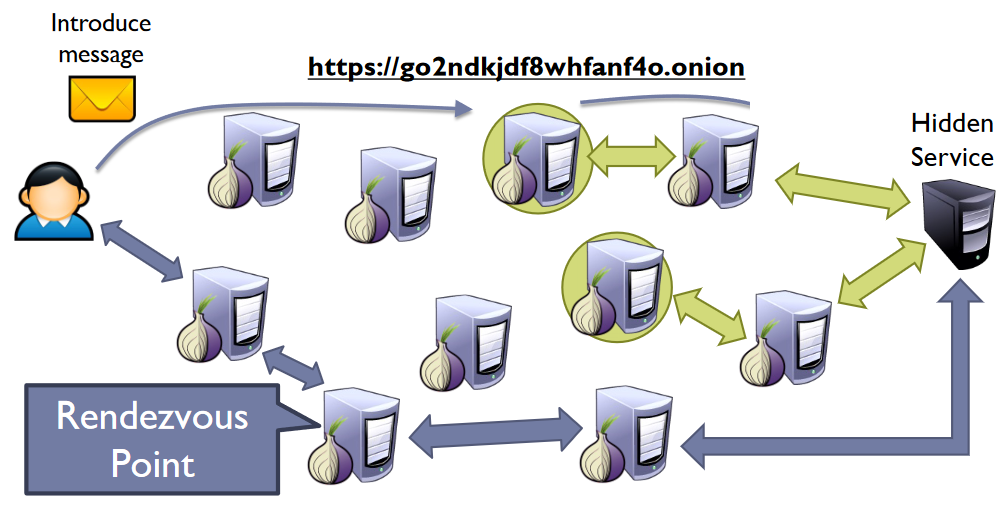
\includegraphics[scale=0.5]{29.png}
\end{figure}
\subsection{Investigation of Tor Traffic}
Onion Routing gets its security from the fact that it is difficult for an adversary to position itself on networks such that it is able to view all the nodes in the route, but if someone is able to learn the entire path, it loses its security. By probing the entry and exit relays, we can correlate
the traffic (e.g., by volume or timing).
\subsubsection{Predecessor Attack}
The investigator controls two relays of the Tor network. Probability of being in the right positions (entry and exit) increases over time.
\begin{figure}[H]
\centering
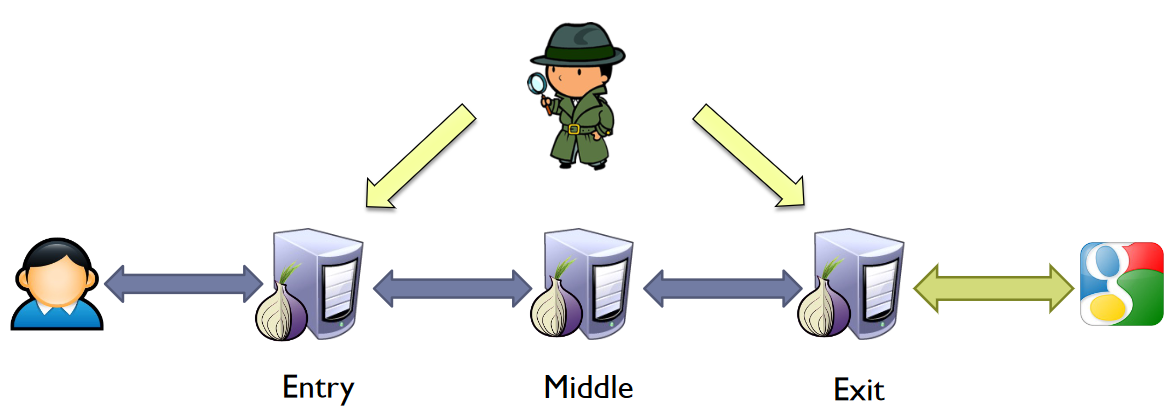
\includegraphics[scale=0.3]{22.png}
\end{figure}
Guard relays help prevent attackers from becoming the first relay. If a user chooses an evil guard, the is a $M/N$ chance of full compromise, where $N$ is the total number of nodes and $M$ is the number of nodes controlled by the attacker.
\subsubsection{Protocol Level Attacks}
Can confirm anonymous communication relationships quickly and accurately by manipulating one single cell.Detection is possible because Tor uses the counter mode AES (AES-CTR) for encrypting cells.
\begin{figure}[H]
\centering
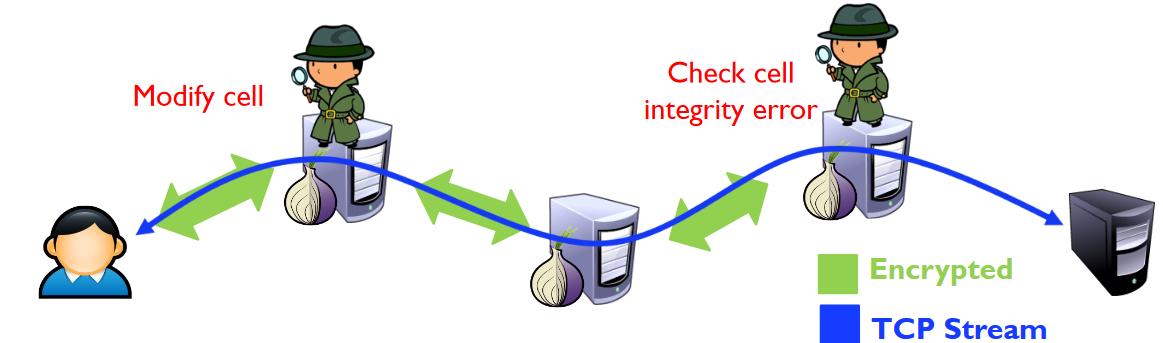
\includegraphics[scale=0.3]{23.png}
\end{figure}
\subsubsection{Eavesdropping On The Exit Node}
Tor does not provide end-to-end encryption. If users don’t use end-to-end encryption, e.g., https, it is possible to eavesdrop on the circuit’s exit node.
\begin{figure}[H]
\centering
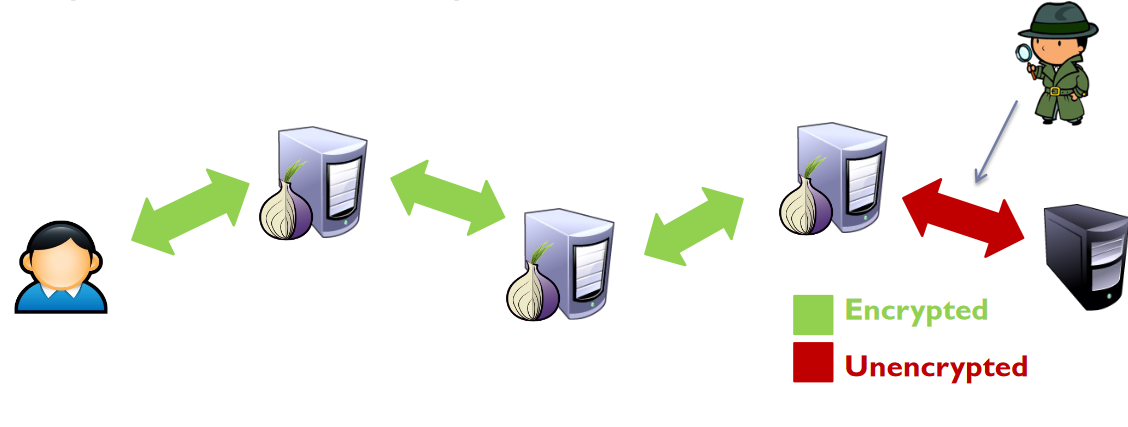
\includegraphics[scale=0.3]{24.png}
\end{figure}
\subsubsection{HTTPS traffic sniffing at exit node}
Tor exit relays tamper with HTTPS connections, e.g., by:
\begin{itemize}
\item Impersonating the destination website with a rogue certificate
\item SSL stripping: downgrade the connection from HTTPS to HTTP
\end{itemize}
\begin{figure}[H]
\centering
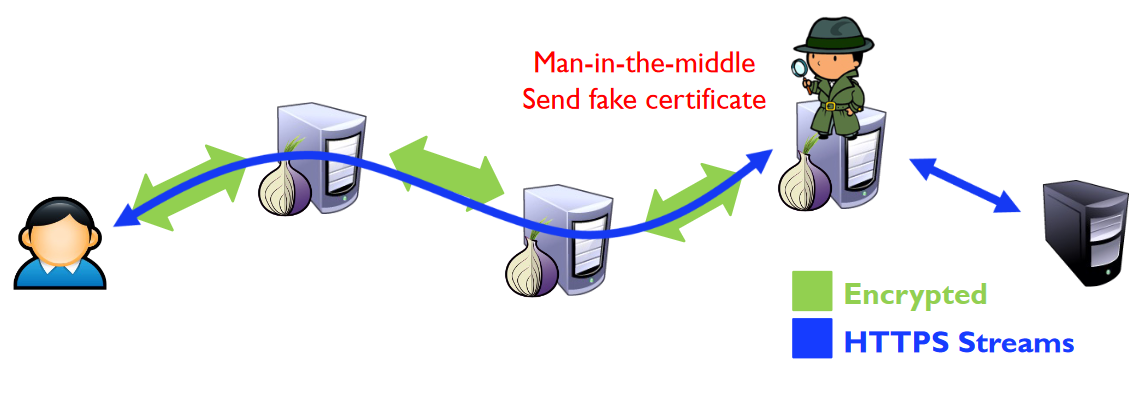
\includegraphics[scale=0.3]{25.png}
\end{figure}
\subsubsection{Tor Traffic Fingerprinting}
A local, passive observer can monitor a web-browsing client’s encrypted traffic to determine its web activity. This also works for hidden services. One can control the Tor entry point for the computer hosting the hidden service and fingerprint it.
\begin{figure}[H]
\centering
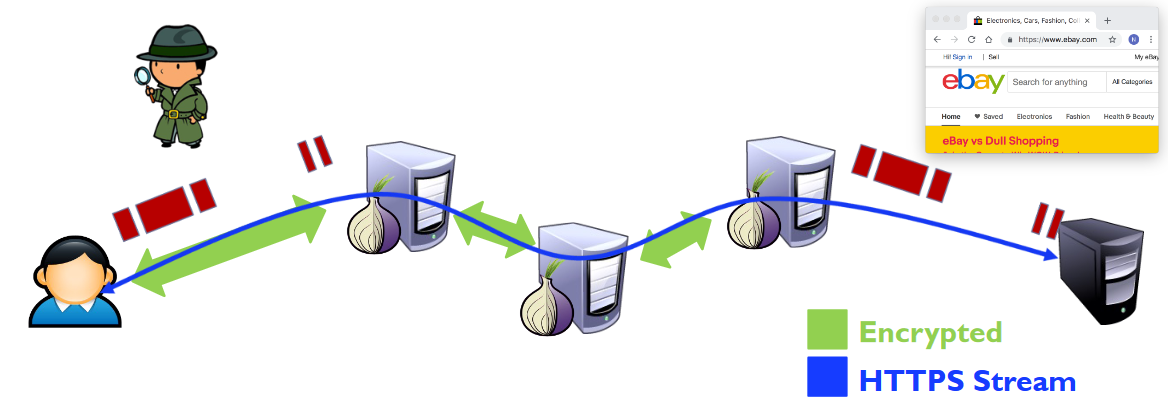
\includegraphics[scale=0.3]{26.png}
\end{figure}
\section{Botnets}
A botnet is a collection of software "robots" hat run on host computers autonomously and automatically, controlled remotely by an attacker or attackers.\\
\\
Botmasters are not necessarily (only) botnet’s end-beneficiaries. They may be paid by advertising companies, or companies that send spam, viruses, or other malware.\\
\\
During a bot’s installation, the malware typically installs what is known as a backdoor, or a program that allows the bot master to communicate, control and install software onto the infected computer.
\subsection{Infecting Botnet Nodes}
The most popular methods of spreading a botnet are:
\begin{itemize}
\item Email
\item Pirated software
\end{itemize}
On the other hand, if one wishes to recruit a botnet, the most popular method is by drive-by download, while visiting a malicious site.
\subsection{Trail Obfuscation Techniques}
Some techniques to obfuscate a botnet's trail are:
\begin{itemize}
\item Piggyback on existing protocols and systems
\item Fast Flux and Domain Generation Algorithms (DGA)
\item P2P botnet architectures
\item Encryption
\item Rootkits
\end{itemize}
Internet Relay Chat (IRC) is often used to facilitate communication in the form of text. An attacker opens private IRC channel on ordinary IRC server and waits for bots to subscribe his own private IRC channel before giving commands.\\
\\
Another option is to use HTTP, where  bots query dedicated web sites regularly for getting new commands.\\
\\
Centralized botnets are easy to implement and have low latency, but are easier to detect and disrupt.
\subsection{Investigating Botnets}
Determining the source of a botnet-based attack is challenging. The classic approach involves an anti-virus scanner, but requires installation on every machine.
\subsubsection{Vertical Detection}
Vertical detection of single bot infections without packet inspection relies on the fact that the botmaster establishes C\&C connections frequently to dessiminate orders. The idea is to use these statistical properties of C\&C communication (periodic behavior) in a machine learning model.
\section{Rootkits}
Exploits are malicious programs that take advantage of application software or OS vulnerabilities. Exploit kits are more comprehensive tools that contain a collection of exploits.\\
\\
The behavior of the operating system can be affected by the presence of rootkits. The goals of a rootkit are:
\begin{itemize}
\item Enable future access to system by attacker
\item Remove evidence of original attack and activity that led to rootkit installation
\item Hide future attacker activity (files, net connections, processes) and prevent it from being logged
\item Install tools to widen scope of penetration
\item Secure system so other attackers can’t take control of system from original attacker
\end{itemize}
\subsection{Rootkit Tools}
Some tools commonly used in rootkits include:
\begin{itemize}
\item Backdoors
\item Packet sniffers
\item Log-wiping utilities
\item DDOS programs
\item IRC programs
\item Password crackers
\item Hiding utilities
\end{itemize}
Some stealth techniques are:
\begin{itemize}
\item File masquerading
\item Hooking
\item Virtualization
\item Direct Kernel Object Manipulation (DKOM)
\end{itemize}
\section{Malware Analysis}
Malware may be analysed for various reasons, including the assessment of damage, identification of vulnerabilities or to aid in finding the perpetrator.
\subsection{Analysis Techniques}
Some static analysis techniques are:
\begin{itemize}
\item Hashing the file
\item Disassembly
\item Decompilation
\end{itemize}
While static analysis will reveal some immediate information, a dynamic analysis  is conducted by observing and manipulating malware as it runs and may reveal more information.
\begin{figure}[H]
\centering
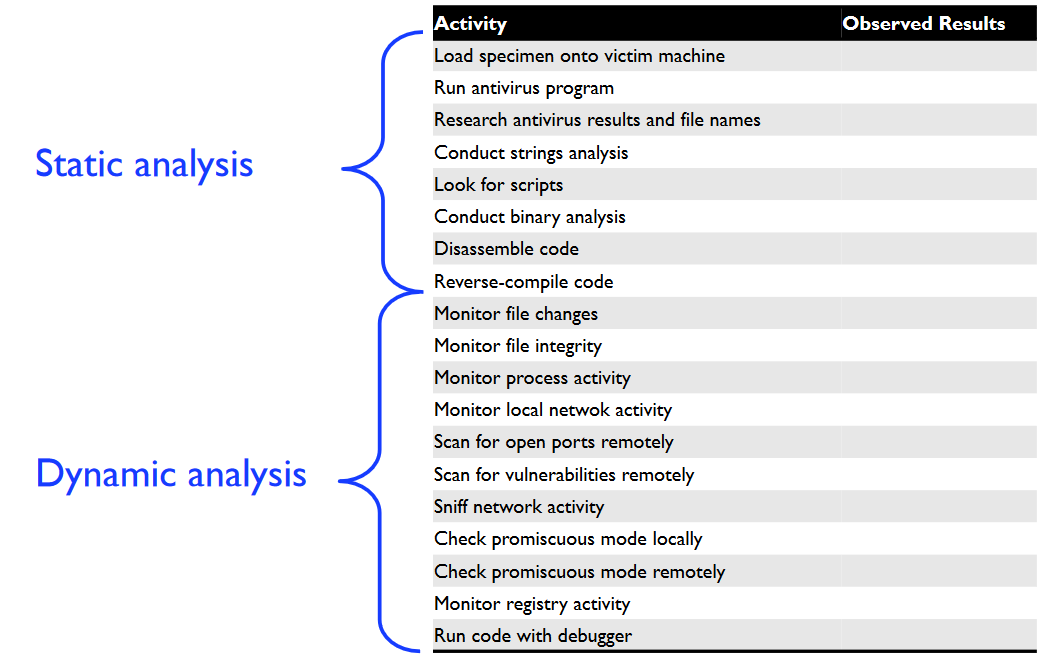
\includegraphics[scale=0.3]{27.png}
\end{figure}
\subsection{Anti-Analysis Techniques}
Some anti-static analysis techniques include opcode obfuscation, imported function ofbuscation and targeted attacks on analysis tools.\\
\\
On the other hand, some anti-dynamic analysis techniques are the detection of virtualization, instrumentation and debuggers.
\subsection{Creating a Safe Environment}
When performing malware analysis it is common practice to use a virtual machine. It is important, however, to set up the machine with no network or host-only network and to take into consideration that no virtualization software is perfect. Malicious code may be able to detect it is running on a virtual environment.
\section{Cryptocurrency Investigations}
Virtual currencies are often used for online transactions.
\subsection{Bitcoin}
In the dark web, bitcoin is frequently used as currency, since it is fully decentralized and more private.\\
\\
In this system, clients are identified by public keys of their choice. Peers of the Bitcoin network connect to each other over an unencrypted TCP channel. There is no authentication in the network, so each node just keeps a list of IP addresses associated with its connections.
\subsubsection{Transaction Graph}
In the transaction graph, the current transaction references previous transactions, called inputs. Other nodes verifying this transaction will check those inputs and through referenced input links, ownership of bitcoins is passed along.\\
\\
To validate a transaction, one must check the entire chain all the way back to the first tx ever made: Transaction history is organized as a chain of blocks, a blockchain.
\subsubsection{Mining}
Mining is the process by which new bitcoin is added to the money supply. Miners are responsible for generating and appending new blocks to the head of the blockchain. Miners provide processing power to the bitcoin network in exchange for the opportunity to be rewarded bitcoin.\\
\\
Miners compete to solve a difficult math problem, based on the cryptographic hash algorithm. The solution to the problem (Proof-of-Work) is included in the block and acts as a proof that the miner solved the problem.
\subsection{Bitcoin Investigations}
Some trail obfuscation techniques present in bitcoin include:
\begin{itemize}
\item Bitcoin address are not mapped to the real user identity
\item Bitcoin transactions don’t contain personal information
\item IP address of client not included in new transactions
\item User can generate as many Bitcoin addresses as needed
\end{itemize}
Altough names are not associated with transactions, their metadata is recorded and publicly avaliable. Some other weaknesses include:
\begin{itemize}
\item Authentication mechanism in Bitcoin service providers may link user IPs to Bitcoin addresses
\item The chain of transactions is transparent and traceable
\item Bitcoin address exposed on the Internet reveal all transactions related to its owner
\item Gathering some or all inputs when sending Bitcoins to others may expose other addresses of the sender
\end{itemize}
Often times, heuristics are also applied, for example, the shared spending or the fresh-change-address heuristics. Shared spending is evidence of joint controlof the different input addresses. Two inputs to the transaction are most likely under the control of the same user:
\begin{figure}[H]
\centering
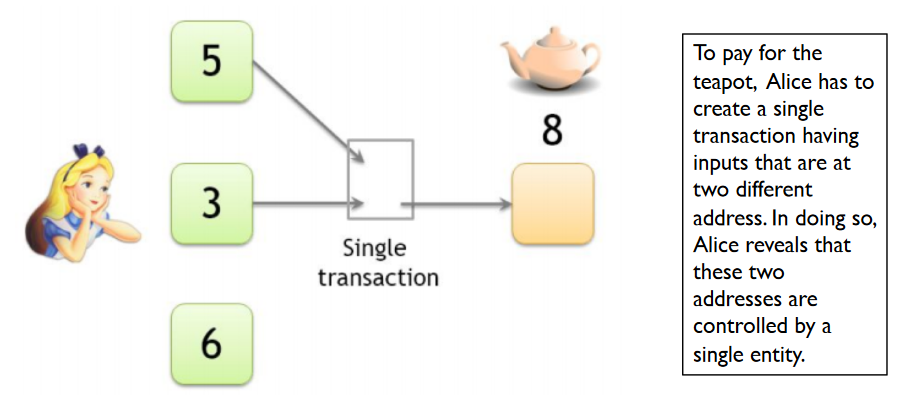
\includegraphics[scale=0.4]{32.png}
\end{figure}
Wallet software typically generate a fresh address whenever a change address is required. Change addresses generally have never before appeared:
\begin{figure}[H]
\centering
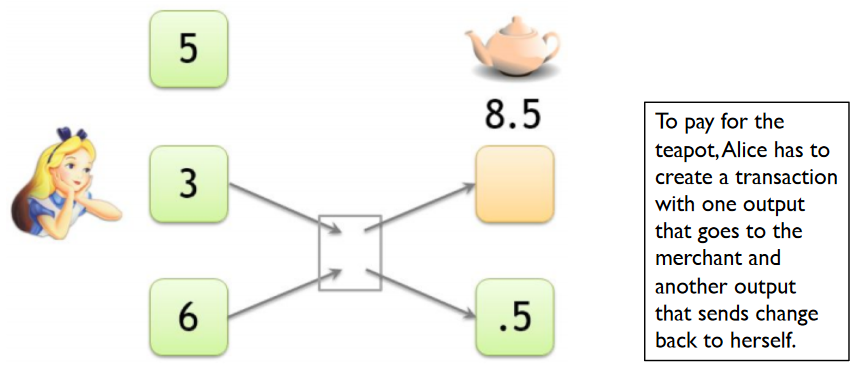
\includegraphics[scale=0.4]{33.png}
\end{figure}
In summary, when investigating bitcoin, one should analyse the transaction graph and the bitcoin protocol and network.
\section{Mobile Forensics}
\subsection{Evidence From Android Devices}
By having the Linux kernel at the heart of its platform, Android tries to ensure security at the OS level. Android devices have two primary types of memory:
\begin{itemize}
\item NAND flash
\item RAM
\end{itemize}
And the sequence of steps on the boot process is as follows:
\begin{itemize}
\item Boot ROM code execution
\item The boot loader
\item The Linux kernel
\item The init process
\item Zygote and Dalvik
\item The system server
\end{itemize}
\subsubsection{Data Storage}
Android apps primarily store data in two locations: internal and external storage (SD card).\\
\\
The internal data of all apps is saved in /data/data/<apppkg>. There are five methods of data storage on a device
\begin{itemize}
\item Shared preferences: this location provides a framework to store key-value pairs of primitive data types in the .xml format
\item Files on internal storage: data stored here is private and cannot be accessed by other applications
\item Files on external storage: files can be stored by the apps in external storage, which does not have strict security enforcement
\item SQLite database: Android SDK provides dedicated APIs that allow developers to use SQLite DBs in their applications
\item Network: The final data storage mechanism available to developers is the network (e.g. Dropbox)
\end{itemize}
\subsection{Evidence Extraction}
\subsubsection{ADB Pull}
The ADB pull command can be used  to pull single files or directories directly from the device. Google implemented ADB backup functionality which allows users (and forensic examiners) to backup app data to local computer over ADB.
\subsubsection{Screen Capture}
Sometimes, taking a picture is the only way to take data off of a phone
\subsubsection{Software-Based Physical Techniques}
It is possible to extract data using an imaging tool (e.g. dd).
\subsubsection{Hardware-Based Physical Techniques}
JTAG interface: used during the device production process to communicate with the processor for testing\\
\\
Chip-off: nvolves heating the device's circuit board until the solder holding the components to the board melts, and then removing the flash memory chip
\subsection{Android App Reverse Engineering}
The reverse engineering of apps enables repackaging attacks. The easy depompilation of DEX bytecode enables source code exposure and the simple distribution of repackaged apps make this a serious issue.
\section{Cloud Forensics}
There ate three main models: IaaS, PaaS, and SaaS. Some challenges when investigating cloud networks are:
\begin{itemize}
\item Storage system is no longer local
\item Each cloud server contains files from multiple users
\item Even if data belonged to a particular subject is identified, separating it from different users is difficult
\item Other than cloud service providers (CSPs), there is usually no evidence that links a given data file to a particular suspect
\end{itemize}
\subsection{Virtual Machines}
Cloud services often rely on the power of virtual machines. This brings some difficulty,  since when we turn off a virtual machine, all the data will be lost if we do not have the
image of the instance.\\
\\
Virtual Machine Introspection (VMI) is the process of externally monitoring the runtime state of VM from either the Virtual Machine Monitor (VMM), or from some virtual machine other than the one being examined.

\end{document}